\documentclass{scrartcl}
\usepackage[utf8]{inputenc}
\usepackage[ngerman,english]{babel}
\usepackage{tabularx}
\usepackage{booktabs}
\usepackage{amsmath}
\usepackage{graphicx}
\usepackage{units}

\usepackage{listings}
\usepackage{fourier}
\usepackage{xcolor}

\lstset{
   backgroundcolor=\color{lightgray},
   basicstyle=\scriptsize\ttfamily,
   keywordstyle=\bfseries\ttfamily\color{orange},
   stringstyle=\color{green}\ttfamily,
   commentstyle=\color{middlegray}\ttfamily,
   emph={square}, 
   emphstyle=\color{blue}\texttt,
   emph={[2]root,base},
   emphstyle={[2]\color{yac}\texttt},
   showstringspaces=false,
   flexiblecolumns=false,
   tabsize=2,
   numbers=left,
   numberstyle=\tiny,
   numberblanklines=false,
   stepnumber=1,
   numbersep=10pt,
   xleftmargin=15pt
 }

\parindent0mm

\renewcommand*\labelitemi{\normalfont\bfseries\textendash}

\title{Merkzettel \LaTeX}
\author{Elke Faßhauer}
\date{DSA Rossleben 2017 \\ CC-BY-SA version 4.0}

\begin{document}

\maketitle

\section{Struktur des Hauptdokumentes}

\begin{itemize}
 \item Wahl Art des Dokumentes mit \lstinline$\documentclass{}$, z.B.
       \lstinline$scrbook$, \lstinline$scrartcl$, \lstinline$beamer$, ...
 \item Einbinden verschiedener Pakete mit \lstinline$\usepackage[]{}$
 \item Inhalt umrahmt von \lstinline$\begin{document} ... \end{document}$
\end{itemize}

\begin{lstlisting}
\documentclass{scrartcl}
\usepackage[utf8]{inputenc}                 % Zeichencodierung
\usepackage{tabularx}                       % Tabellen
\usepackage{booktabs}                       % eleganter formatierte Tabellen
\usepackage{amsmath,amsfonts,amssymb}       % Matheumgebung und Symbole
\usepackage{graphicx}                       % Grafiken
\usepackage{units}                          % Setzen von Werten mit Einheiten
\usepackage{ngerman}                        % Verwende deutschen Zeilenumbruch

\begin{document}
 Inhalt
\end{document}
\end{lstlisting}

Der Inhalt kann, muss aber nicht im gleichen Dokument zu finden sein. Ab einer
Gesamtlänge des kompilierten Inhaltes von einer Seite, empfiehlt es sich, den Inhalt
in andere Dateien auszulagern und diese mit \lstinline$\input{}$ oder
\lstinline$\include{}$ einzubinden:

\begin{lstlisting}
%allerlei Pakete

\begin{document}

 \section{Struktur des Hauptdokumentes}

\begin{itemize}
 \item Wahl Art des Dokumentes mit \lstinline$\documentclass{}$, z.B.
       \lstinline$scrbook$, \lstinline$scrartcl$, \lstinline$beamer$, ...
 \item Einbinden verschiedener Pakete mit \lstinline$\usepackage[]{}$
 \item Inhalt umrahmt von \lstinline$\begin{document} ... \end{document}$
\end{itemize}

\begin{lstlisting}
\documentclass{scrartcl}
\usepackage[utf8]{inputenc}                 % Zeichencodierung
\usepackage{tabularx}                       % Tabellen
\usepackage{booktabs}                       % eleganter formatierte Tabellen
\usepackage{amsmath,amsfonts,amssymb}       % Matheumgebung und Symbole
\usepackage{graphicx}                       % Grafiken
\usepackage{units}                          % Setzen von Werten mit Einheiten
\usepackage{ngerman}                        % Verwende deutschen Zeilenumbruch

\begin{document}
 Inhalt
\end{document}
\end{lstlisting}

Der Inhalt kann, muss aber nicht im gleichen Dokument zu finden sein. Ab einer
Gesamtlänge des kompilierten Inhaltes von einer Seite, empfiehlt es sich, den Inhalt
in andere Dateien auszulagern und diese mit \lstinline$\input{}$ oder
\lstinline$\include{}$ einzubinden:

\begin{lstlisting}
%allerlei Pakete

\begin{document}

 \section{Struktur des Hauptdokumentes}

\begin{itemize}
 \item Wahl Art des Dokumentes mit \lstinline$\documentclass{}$, z.B.
       \lstinline$scrbook$, \lstinline$scrartcl$, \lstinline$beamer$, ...
 \item Einbinden verschiedener Pakete mit \lstinline$\usepackage[]{}$
 \item Inhalt umrahmt von \lstinline$\begin{document} ... \end{document}$
\end{itemize}

\begin{lstlisting}
\documentclass{scrartcl}
\usepackage[utf8]{inputenc}                 % Zeichencodierung
\usepackage{tabularx}                       % Tabellen
\usepackage{booktabs}                       % eleganter formatierte Tabellen
\usepackage{amsmath,amsfonts,amssymb}       % Matheumgebung und Symbole
\usepackage{graphicx}                       % Grafiken
\usepackage{units}                          % Setzen von Werten mit Einheiten
\usepackage{ngerman}                        % Verwende deutschen Zeilenumbruch

\begin{document}
 Inhalt
\end{document}
\end{lstlisting}

Der Inhalt kann, muss aber nicht im gleichen Dokument zu finden sein. Ab einer
Gesamtlänge des kompilierten Inhaltes von einer Seite, empfiehlt es sich, den Inhalt
in andere Dateien auszulagern und diese mit \lstinline$\input{}$ oder
\lstinline$\include{}$ einzubinden:

\begin{lstlisting}
%allerlei Pakete

\begin{document}

 \input{hauptdokument}                  % Datei hauptdokument.tex einfuegen
 \include{hauptdokument}                % auf neuer Seite einfuegen

\end{document}

\end{lstlisting}
                  % Datei hauptdokument.tex einfuegen
 \section{Struktur des Hauptdokumentes}

\begin{itemize}
 \item Wahl Art des Dokumentes mit \lstinline$\documentclass{}$, z.B.
       \lstinline$scrbook$, \lstinline$scrartcl$, \lstinline$beamer$, ...
 \item Einbinden verschiedener Pakete mit \lstinline$\usepackage[]{}$
 \item Inhalt umrahmt von \lstinline$\begin{document} ... \end{document}$
\end{itemize}

\begin{lstlisting}
\documentclass{scrartcl}
\usepackage[utf8]{inputenc}                 % Zeichencodierung
\usepackage{tabularx}                       % Tabellen
\usepackage{booktabs}                       % eleganter formatierte Tabellen
\usepackage{amsmath,amsfonts,amssymb}       % Matheumgebung und Symbole
\usepackage{graphicx}                       % Grafiken
\usepackage{units}                          % Setzen von Werten mit Einheiten
\usepackage{ngerman}                        % Verwende deutschen Zeilenumbruch

\begin{document}
 Inhalt
\end{document}
\end{lstlisting}

Der Inhalt kann, muss aber nicht im gleichen Dokument zu finden sein. Ab einer
Gesamtlänge des kompilierten Inhaltes von einer Seite, empfiehlt es sich, den Inhalt
in andere Dateien auszulagern und diese mit \lstinline$\input{}$ oder
\lstinline$\include{}$ einzubinden:

\begin{lstlisting}
%allerlei Pakete

\begin{document}

 \input{hauptdokument}                  % Datei hauptdokument.tex einfuegen
 \include{hauptdokument}                % auf neuer Seite einfuegen

\end{document}

\end{lstlisting}
                % auf neuer Seite einfuegen

\end{document}

\end{lstlisting}
                  % Datei hauptdokument.tex einfuegen
 \section{Struktur des Hauptdokumentes}

\begin{itemize}
 \item Wahl Art des Dokumentes mit \lstinline$\documentclass{}$, z.B.
       \lstinline$scrbook$, \lstinline$scrartcl$, \lstinline$beamer$, ...
 \item Einbinden verschiedener Pakete mit \lstinline$\usepackage[]{}$
 \item Inhalt umrahmt von \lstinline$\begin{document} ... \end{document}$
\end{itemize}

\begin{lstlisting}
\documentclass{scrartcl}
\usepackage[utf8]{inputenc}                 % Zeichencodierung
\usepackage{tabularx}                       % Tabellen
\usepackage{booktabs}                       % eleganter formatierte Tabellen
\usepackage{amsmath,amsfonts,amssymb}       % Matheumgebung und Symbole
\usepackage{graphicx}                       % Grafiken
\usepackage{units}                          % Setzen von Werten mit Einheiten
\usepackage{ngerman}                        % Verwende deutschen Zeilenumbruch

\begin{document}
 Inhalt
\end{document}
\end{lstlisting}

Der Inhalt kann, muss aber nicht im gleichen Dokument zu finden sein. Ab einer
Gesamtlänge des kompilierten Inhaltes von einer Seite, empfiehlt es sich, den Inhalt
in andere Dateien auszulagern und diese mit \lstinline$\input{}$ oder
\lstinline$\include{}$ einzubinden:

\begin{lstlisting}
%allerlei Pakete

\begin{document}

 \section{Struktur des Hauptdokumentes}

\begin{itemize}
 \item Wahl Art des Dokumentes mit \lstinline$\documentclass{}$, z.B.
       \lstinline$scrbook$, \lstinline$scrartcl$, \lstinline$beamer$, ...
 \item Einbinden verschiedener Pakete mit \lstinline$\usepackage[]{}$
 \item Inhalt umrahmt von \lstinline$\begin{document} ... \end{document}$
\end{itemize}

\begin{lstlisting}
\documentclass{scrartcl}
\usepackage[utf8]{inputenc}                 % Zeichencodierung
\usepackage{tabularx}                       % Tabellen
\usepackage{booktabs}                       % eleganter formatierte Tabellen
\usepackage{amsmath,amsfonts,amssymb}       % Matheumgebung und Symbole
\usepackage{graphicx}                       % Grafiken
\usepackage{units}                          % Setzen von Werten mit Einheiten
\usepackage{ngerman}                        % Verwende deutschen Zeilenumbruch

\begin{document}
 Inhalt
\end{document}
\end{lstlisting}

Der Inhalt kann, muss aber nicht im gleichen Dokument zu finden sein. Ab einer
Gesamtlänge des kompilierten Inhaltes von einer Seite, empfiehlt es sich, den Inhalt
in andere Dateien auszulagern und diese mit \lstinline$\input{}$ oder
\lstinline$\include{}$ einzubinden:

\begin{lstlisting}
%allerlei Pakete

\begin{document}

 \input{hauptdokument}                  % Datei hauptdokument.tex einfuegen
 \include{hauptdokument}                % auf neuer Seite einfuegen

\end{document}

\end{lstlisting}
                  % Datei hauptdokument.tex einfuegen
 \section{Struktur des Hauptdokumentes}

\begin{itemize}
 \item Wahl Art des Dokumentes mit \lstinline$\documentclass{}$, z.B.
       \lstinline$scrbook$, \lstinline$scrartcl$, \lstinline$beamer$, ...
 \item Einbinden verschiedener Pakete mit \lstinline$\usepackage[]{}$
 \item Inhalt umrahmt von \lstinline$\begin{document} ... \end{document}$
\end{itemize}

\begin{lstlisting}
\documentclass{scrartcl}
\usepackage[utf8]{inputenc}                 % Zeichencodierung
\usepackage{tabularx}                       % Tabellen
\usepackage{booktabs}                       % eleganter formatierte Tabellen
\usepackage{amsmath,amsfonts,amssymb}       % Matheumgebung und Symbole
\usepackage{graphicx}                       % Grafiken
\usepackage{units}                          % Setzen von Werten mit Einheiten
\usepackage{ngerman}                        % Verwende deutschen Zeilenumbruch

\begin{document}
 Inhalt
\end{document}
\end{lstlisting}

Der Inhalt kann, muss aber nicht im gleichen Dokument zu finden sein. Ab einer
Gesamtlänge des kompilierten Inhaltes von einer Seite, empfiehlt es sich, den Inhalt
in andere Dateien auszulagern und diese mit \lstinline$\input{}$ oder
\lstinline$\include{}$ einzubinden:

\begin{lstlisting}
%allerlei Pakete

\begin{document}

 \input{hauptdokument}                  % Datei hauptdokument.tex einfuegen
 \include{hauptdokument}                % auf neuer Seite einfuegen

\end{document}

\end{lstlisting}
                % auf neuer Seite einfuegen

\end{document}

\end{lstlisting}
                % auf neuer Seite einfuegen

\end{document}

\end{lstlisting}

\section{Kapitel, Abschnitte, Unterabschnitte ...}

\begin{itemize}
 \item Kapitel: \lstinline$\chapter{Kapiteltitel}$
 \item Abschnitt: \lstinline$\section{}$
 \item Unterabschnitt: \lstinline$\subsection{}$
\end{itemize}

\begin{lstlisting}
\section{Ein Abschnitt mit Nummerierung}
\section*{Ein Abschnitt ohne Nummerierung}
 \subsection{Ein Unterabschnitt}
 \subsection*{Ein Unterabschnitt ohne Nummerierung}
\end{lstlisting}

Auf diesem Merkzettel sind \emph{Struktur des Hauptdokumentes},
\emph{Kapitel, Abschnitt, Unterabschnitte} usw. \lstinline$\section{}$
und \emph{Chemische Formeln im Fließtext} ist eine \lstinline$\subsection{}$.

\section{Formelsatz}

\subsection*{In einer Formelumgebung}
abgesetzte, (nummerierte), referenzierbare Formel

\begin{lstlisting}
\begin{equation}
 \label{Satz_des_Pythagoras}      % optional
 a^2 + b^2 = c^2
\end{equation}
\end{lstlisting}

\begin{equation}
 \label{Satz_des_Pythagoras}      % optional
 a^2 + b^2 = c^2
\end{equation}

\begin{lstlisting}
\begin{equation*}
 c \le a + b
\end{equation*}
\end{lstlisting}

\begin{equation*}
 c \le a + b
\end{equation*}

\subsection*{Im Fließtext}
Einrahmung der Formel durch \$Formel\$

\begin{lstlisting}
Aus dem Satz des Pythagoras (siehe Gleichung \ref{Satz_des_Pythagoras}) laesst
sich die Laenge der Hypotenuse zu $c = \sqrt{a^2 + b^2}$ bestimmen.
\end{lstlisting}

Aus dem Satz des Pythagoras (siehe Gleichung \ref{Satz_des_Pythagoras}) lässt
sich die Länge der Hypotenuse zu $c = \sqrt{a^2 + b^2}$ bestimmen.


\subsection{Chemische Formeln im Fließtext}
\begin{itemize}
 \item Elementsymbole werden in normaler Schrift geschrieben: H, C, O, N, Xe, ...
 \item Anzahlen und Ladungen werden in der Matheumgebung notiert
\end{itemize}

\begin{lstlisting}
Bei der Autoprotolyse des Wassers entstehen Hydroniumionen H$_{3}$O$^{+}$ und
Hydroxidionen OH$^{-}$.
\end{lstlisting}

Bei der Autoprotolyse des Wassers entstehen Hydroniumionen H$_{3}$O$^{+}$ und
Hydroxidionen OH$^{-}$.


\section{Aufzählungen}

\subsection{Nummeriert}
\begin{lstlisting}
\begin{enumerate}
 \item erster Punkt
 \item zweiter Punkt
\end{enumerate}
\end{lstlisting}

\begin{enumerate}
 \item erster Punkt
 \item zweiter Punkt
\end{enumerate}

\subsection{Symbole}
\begin{lstlisting}
\begin{itemize}
 \item erster Punkt
 \item zweiter Punkt
\end{itemize}
\end{lstlisting}

\begin{itemize}
 \item erster Punkt
 \item zweiter Punkt
\end{itemize}

\section{Tabellen}
Tabellen befinden sich in Tabellenumgebungenen, die
aus mehreren Elementen bestehen. Sie haben:

\begin{itemize}
 \item eine Überschrift \lstinline$\caption{}$
 \item ein Label (auf alle(!) Tabellen muss im Text verwiesen werden)
       \lstinline$\label{}$
 \item die Tabelle selbst
 \begin{itemize}
  \item Anzahl der Spalten, die jeweils linksbündig \lstinline$l$, zentriert
        \lstinline$c$ oder rechtsbündig \lstinline$r$ sein können
  \item Spalten werden mit \lstinline$&$ getrennt
  \item am Ende jeder Zeile steht \lstinline$\\$
 \end{itemize}
\end{itemize}

\begin{lstlisting}
\begin{table}[h]
 \caption{Dieses ist unsere Beispieltabelle. Der Inhalt ist weder relevant noch
          zutreffend.}
 \centering
 \begin{tabular}{lcr} % drei Spalten
  \toprule
   Kurs      & blaue Augen & braune Augen\\
  \midrule
   5.1       & 4           & 10\\
   5.2       & 7           & 9\\
   5.3       & 15          & 1\\
  \bottomrule
 \end{tabular}
 \label{table:beispiel}
\end{table}
\end{lstlisting}

\begin{table}[h]
 \caption{Dieses ist unsere Beispieltabelle. Der Inhalt ist weder relevant noch
          zutreffend.}
 \centering
 \begin{tabular}{lcr} % drei Spalten
  \toprule
   Kurs      & blaue Augen & braune Augen\\
  \midrule
   5.1       & 4           & 10\\
   5.2       & 7           & 9\\
   5.3       & 15          & 1\\
  \bottomrule
 \end{tabular}
 \label{table:beispiel}
\end{table}

\danger Für den Fall der SchülerAkademie muss \lstinline$\table$ durch
        \textbf{\textbackslash dsatable} ersetzt werden. Desweiteren ist die
        Option \lstinline$[h]$ im DSA-template nicht zulässig. Sie sollte
        einfach weggelassen werden.

\section{Abbildungen}
Abbildungen befinden sich in Abbildungsumgebungenen, die
aus mehreren Elementen bestehen. Sie haben:

\begin{itemize}
 \item die Abbildung selbst
 \item eine Unterschrift \lstinline$\caption{}$
 \item ein Label (auf alle(!) Abbildungen muss im Text verwiesen werden)
       \lstinline$\label{}$
\end{itemize}

\begin{lstlisting}
\begin{figure}[h]
 \centering
 \includegraphics[scale=0.02]{HOMO1-Butadien.png}
 \caption{HOMO des Buta-1,3-dien.}
 \label{figure:beispiel}
\end{figure}
\end{lstlisting}

\begin{figure}[h]
 \centering
 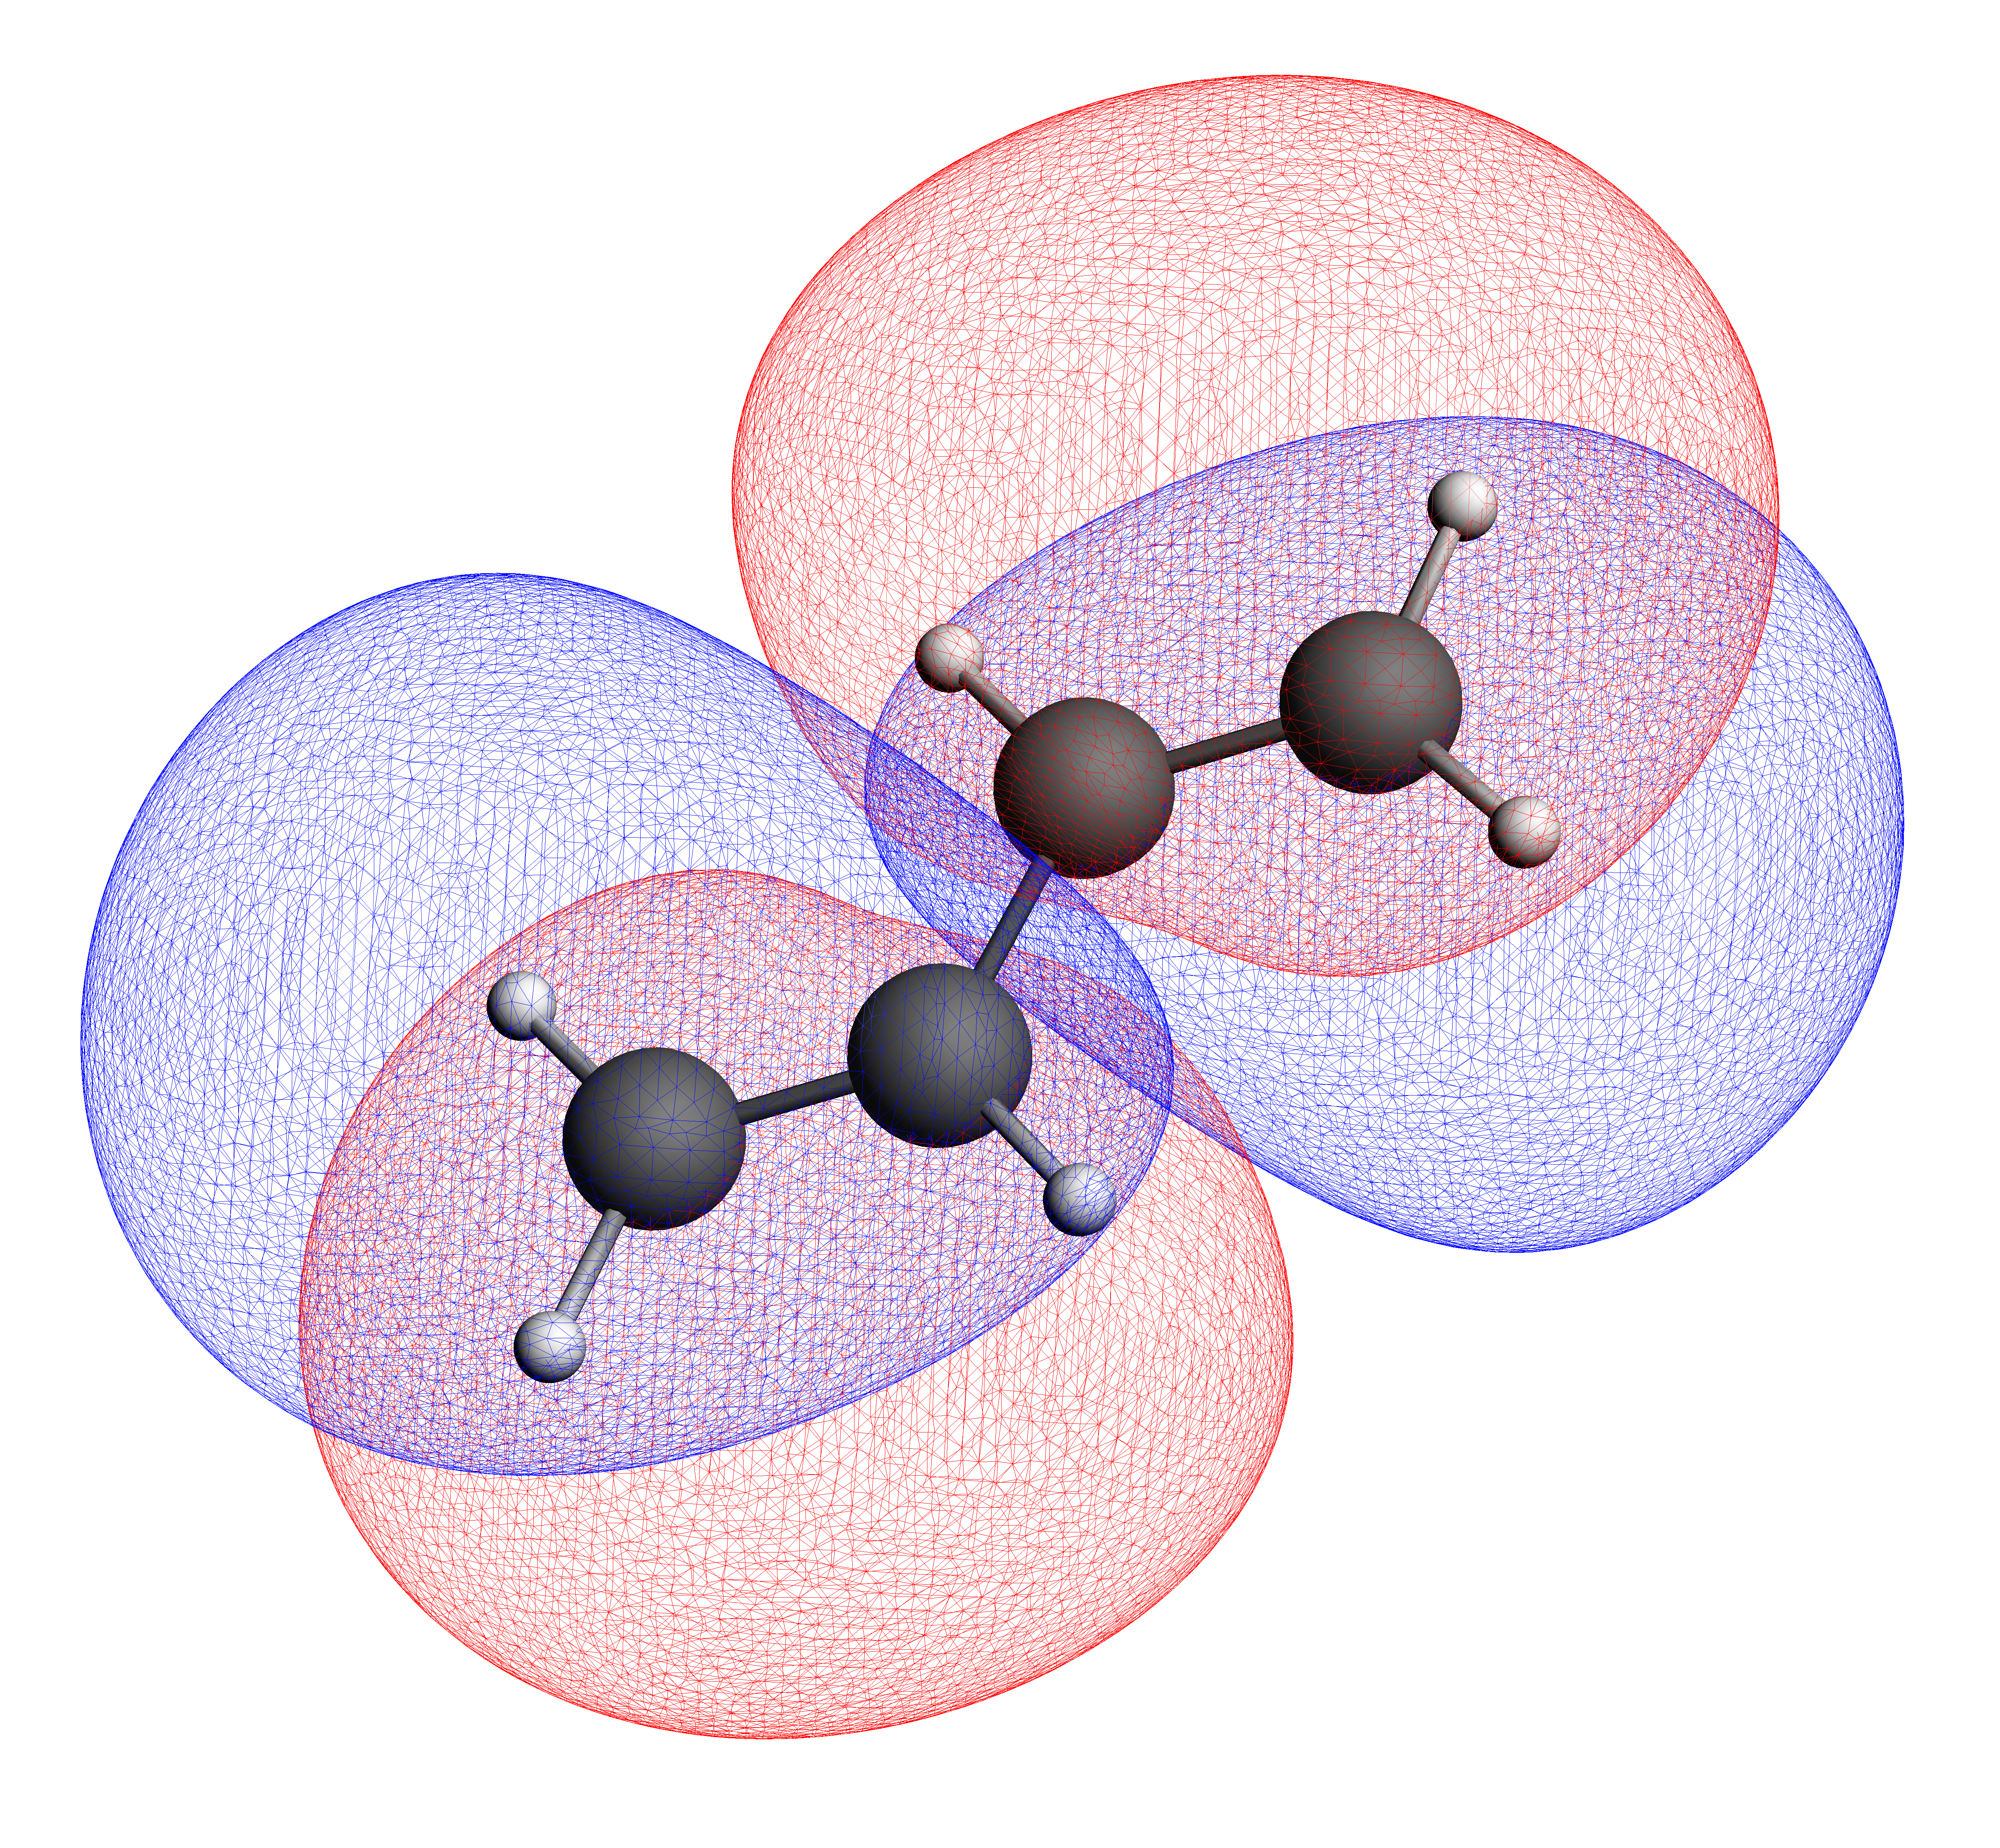
\includegraphics[scale=0.02]{HOMO1-Buten.png}
 \caption{HOMO des Buta-1,2-dien.}
 \label{figure:beispiel}
\end{figure}

\section{Verweise auf Tabellen, Abbildungen, Formeln ...}

\begin{itemize}
 \item jedes Objekt (Tabellen und Abbildungen)
       bekommt ein eindeutiges Label \lstinline$\label{}$,
       Abschnitte und Formeln können ein Label haben
 \item auf dieses kann mit Hilfe von \lstinline$\ref{}$ verwiesen werden
\end{itemize}

\begin{lstlisting}
Wir haben schon einige Objekte und Formeln mit Labeln in den
anderen Abschnitten gesehen, so wie z.B. Tabelle \ref{table:beispiel},
Abbildung \ref{figure:beispiel} oder Gleichung \ref{Satz_des_Pythagoras}.
\end{lstlisting}

Wir haben schon einige Objekte und Formeln mit Labeln in den anderen Abschnitten
gesehen, so wie z.B. Tabelle \ref{table:beispiel}, Abbildung \ref{figure:beispiel}
oder Gleichung \ref{Satz_des_Pythagoras}.


\section{Zitieren mit bibtex}

\begin{itemize}
 \item Einträge in Name.bib Datei verwalten
 \item Literaturbibliothek in Hauptdatei einbauen
 \item mit \lstinline$\cite{}$ zitieren
\end{itemize}

Hauptdatei:
\begin{lstlisting}
%Pakete, Inhalte, usw.
\section{Zitieren mit bibtex}

\begin{itemize}
 \item Einträge in Name.bib Datei verwalten
 \item Literaturbibliothek in Hauptdatei einbauen
 \item mit \lstinline$\cite{}$ zitieren
\end{itemize}

Hauptdatei:
\begin{lstlisting}
%Pakete, Inhalte, usw.
\section{Zitieren mit bibtex}

\begin{itemize}
 \item Einträge in Name.bib Datei verwalten
 \item Literaturbibliothek in Hauptdatei einbauen
 \item mit \lstinline$\cite{}$ zitieren
\end{itemize}

Hauptdatei:
\begin{lstlisting}
%Pakete, Inhalte, usw.
\input{zitieren}

\bibliographystyle{unsrtdin}
\bibliography{lit2}

\end{document}
\end{lstlisting}

Bibliothekendatei Name.bib (hier lit2.bib)
\begin{lstlisting}
@ARTICLE{Fasshauer13,
  author = {Fasshauer, E. and Pernpointner, M. and Gokhberg, K.},
  title = {Interatomic Decay of Inner-Valence Ionized States in ArXe Clusters:
        Relativistic Approach},
  journal = {J. Chem. Phys.},
  year = {2013},
  volume = {138},
  pages = {014305},
}

@BOOK{SakuraiModern94,
  title = {Modern Quantum Mechanics},
  publisher = {Addison-Wesley},
  year = {1994},
  editor = {Tuan, S. F.},
  author = {Sakurai, J. J.},
  edition = {Rev.},
}

@MISC{Nobelpreis,
  author = {Various Artist},
  title = {Development of the metathesis method in organic synthesis},
        url = {http://www.nobelprize.org/nobel\_prizes/chemistry/laureates/2005/advanced-chemistryprize2005.pdf},
        howpublished = {http://www.nobelprize.org/nobel\_prizes/ chemistry/laureates/2005/advanced-chemistryprize2005.pdf},
}
\end{lstlisting}

\begin{lstlisting}
Diese Eintraege sind im Fliesstext selber nicht zu sehen. Wenn man jedoch das
Buch \cite{SakuraiModern94}, den Artikel \cite{Fasshauer13} 
oder den Onlineartikel \cite{Nobelpreis} zitiert,
werden die Nummern automatisch eingefuegt und ein Literaturverzeichnis am Ende
des Dokumentes erstellt.
\end{lstlisting}

Diese Einträge sind im Fließtext selber nicht zu sehen. Wenn man jedoch das
Buch \cite{SakuraiModern94}, den Artikel \cite{Fasshauer13} oder den
Onlineartikel \cite{Nobelpreis} zitiert,
werden die Nummern automatisch eingefügt und ein Literaturverzeichnis am Ende
des Dokumentes erstellt.


\bibliographystyle{unsrtdin}
\bibliography{lit2}

\end{document}
\end{lstlisting}

Bibliothekendatei Name.bib (hier lit2.bib)
\begin{lstlisting}
@ARTICLE{Fasshauer13,
  author = {Fasshauer, E. and Pernpointner, M. and Gokhberg, K.},
  title = {Interatomic Decay of Inner-Valence Ionized States in ArXe Clusters:
        Relativistic Approach},
  journal = {J. Chem. Phys.},
  year = {2013},
  volume = {138},
  pages = {014305},
}

@BOOK{SakuraiModern94,
  title = {Modern Quantum Mechanics},
  publisher = {Addison-Wesley},
  year = {1994},
  editor = {Tuan, S. F.},
  author = {Sakurai, J. J.},
  edition = {Rev.},
}

@MISC{Nobelpreis,
  author = {Various Artist},
  title = {Development of the metathesis method in organic synthesis},
        url = {http://www.nobelprize.org/nobel\_prizes/chemistry/laureates/2005/advanced-chemistryprize2005.pdf},
        howpublished = {http://www.nobelprize.org/nobel\_prizes/ chemistry/laureates/2005/advanced-chemistryprize2005.pdf},
}
\end{lstlisting}

\begin{lstlisting}
Diese Eintraege sind im Fliesstext selber nicht zu sehen. Wenn man jedoch das
Buch \cite{SakuraiModern94}, den Artikel \cite{Fasshauer13} 
oder den Onlineartikel \cite{Nobelpreis} zitiert,
werden die Nummern automatisch eingefuegt und ein Literaturverzeichnis am Ende
des Dokumentes erstellt.
\end{lstlisting}

Diese Einträge sind im Fließtext selber nicht zu sehen. Wenn man jedoch das
Buch \cite{SakuraiModern94}, den Artikel \cite{Fasshauer13} oder den
Onlineartikel \cite{Nobelpreis} zitiert,
werden die Nummern automatisch eingefügt und ein Literaturverzeichnis am Ende
des Dokumentes erstellt.


\bibliographystyle{unsrtdin}
\bibliography{lit2}

\end{document}
\end{lstlisting}

Bibliothekendatei Name.bib (hier lit2.bib)
\begin{lstlisting}
@ARTICLE{Fasshauer13,
  author = {Fasshauer, E. and Pernpointner, M. and Gokhberg, K.},
  title = {Interatomic Decay of Inner-Valence Ionized States in ArXe Clusters:
        Relativistic Approach},
  journal = {J. Chem. Phys.},
  year = {2013},
  volume = {138},
  pages = {014305},
}

@BOOK{SakuraiModern94,
  title = {Modern Quantum Mechanics},
  publisher = {Addison-Wesley},
  year = {1994},
  editor = {Tuan, S. F.},
  author = {Sakurai, J. J.},
  edition = {Rev.},
}

@MISC{Nobelpreis,
  author = {Various Artist},
  title = {Development of the metathesis method in organic synthesis},
        url = {http://www.nobelprize.org/nobel\_prizes/chemistry/laureates/2005/advanced-chemistryprize2005.pdf},
        howpublished = {http://www.nobelprize.org/nobel\_prizes/ chemistry/laureates/2005/advanced-chemistryprize2005.pdf},
}
\end{lstlisting}

\begin{lstlisting}
Diese Eintraege sind im Fliesstext selber nicht zu sehen. Wenn man jedoch das
Buch \cite{SakuraiModern94}, den Artikel \cite{Fasshauer13} 
oder den Onlineartikel \cite{Nobelpreis} zitiert,
werden die Nummern automatisch eingefuegt und ein Literaturverzeichnis am Ende
des Dokumentes erstellt.
\end{lstlisting}

Diese Einträge sind im Fließtext selber nicht zu sehen. Wenn man jedoch das
Buch \cite{SakuraiModern94}, den Artikel \cite{Fasshauer13} oder den
Onlineartikel \cite{Nobelpreis} zitiert,
werden die Nummern automatisch eingefügt und ein Literaturverzeichnis am Ende
des Dokumentes erstellt.


\bibliographystyle{jcpsty_deutsch}
\bibliography{lit2}

\end{document}
